Para realizar la experimentación pedida por el enunciado, se utilizó la tabla \textit{Competidor}. Primero se precedió a vaciar la tabla y a agregarle cinco \textit{Shards} con cinco \textit{replicas} cada uno, obteniendo un total de veinte y cinco \textit{replicas}.

Buscando en la documentación de \textit{RethinkDB}, para que los registros queden balanceados en los distintos \textit{Shards}, hay que utilizar la funcion \textit{rebalance()} sobre la tabla ya que cuando se insertan registros, mismo utilizando un nodo proxy, los mismos NO son insertados en el cluster con ningún algorítmo exacto ni heurístico de balanceo, por lo que los registros terminan siempre insertandoce en un mismo nodo del cluster y es preciso rebalancear el mismo. \\

Se implementó un script python que se encarga de ir insertando documentos a la tabla \textit{Competidor} y cada 100 documentos insertados realiza un rebalanceo de los mismo en el cluster y se toma una medición de cuantos documentos hay en cada nodos para poder analizar como interactuan los servidores para balancear los documentos a medida que aumenta la cantidad. La \ref{fig: cluster} Muestra como se fue balanceando el cluster a medida que se van insertando documentos hasta llegar a una totalidad de diez mil documentos insertados. \\

\begin{figure}[H]
  \centering
    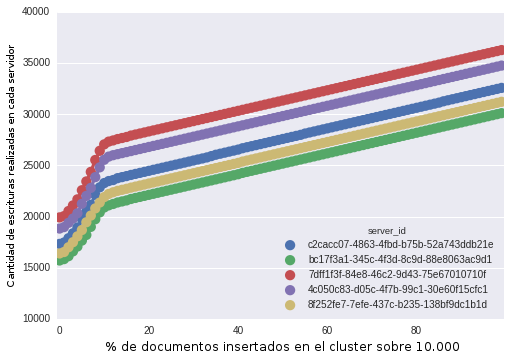
\includegraphics[scale=0.6]{../graficos/cluster.png}
  \caption{Balanceo de documentos en un cluster \textit{RethinkDB} de 5 nodos a medida que se insertan documentos al mismo.}
  \label{fig: cluster}
\end{figure}

En la figura se ve que la curva está dividida en dos partes, hasta más o meno el punto donde el $15\%$ de los diez mil documentos fueron insertados, la curva tiene un crecimiento más acelerado, luego cambia la pendiente. Creemos que esto se debe a la forma en que se balancean los datos, es probable, que cuando no hay muchos documentos, la heurística utilizada para balancear le cueste más conseguir estabilizar el cluster ya que pocas inserciones representan mucho desbalanceo, mientras que cuando hay muchos documentos en el cluster se necesita insertar demasiados documentos extras para lograr desbalancearlo. Es por esto que resulta más costoso balancear pocos documentos realizando muchas operaciónes de escritura, luego de una cierta cantidad de documentos insertados (~$15\%$), el algoritmo se estabiliza y tiene menos necesidad de relizar grandes cambios. \\

Por otro lado, se puede ver que el algoritmo intracluster de balanceo de los datos funciona muy bien, ya que los clusters tienen todos el mismo crecimiento de escritura de documentos sin que se generen grandes desbalanceos. \\